% !TeX spellcheck = <none>
\documentclass[a4paper, 10pt]{scrartcl}  

\usepackage[width=17.00cm, height=25.00cm]{geometry}
\geometry{verbose,a4paper,tmargin=20mm,bmargin=20mm,lmargin=20mm,rmargin=20mm}

\usepackage[english]{babel}
\usepackage[utf8]{inputenc}
\usepackage{tgcursor}
\usepackage{color, colortbl}
\usepackage{amsmath,amssymb,amstext}
\usepackage{tikz}
\usepackage{listings}
\usepackage{graphicx}
\usepackage{scrextend}
\usepackage[colorlinks, 				% Inhaltsverzeichnis verlinken
			pdfpagelabels,
			pdfstartview = FitH,
			bookmarksopen = true,
			bookmarksnumbered = true,
			linkcolor = blue!40!black,
			plainpages = false,
			hypertexnames = false,
			citecolor = black] {hyperref}
\usepackage{array}
\usepackage{tcolorbox}
\usepackage{trfsigns}
\usepackage{transparent}
\usepackage{eso-pic}


\setcounter{tocdepth}{3}  
\setlength{\arrayrulewidth}{0.1pt}
\setlength{\parindent}{0pt}

% Umrahmung definieren
\tcbset{fonttitle=\bfseries, colback=black!1!,colframe=green!50!black!40!}

\begin{document}
	\begin{titlepage}
		\AddToShipoutPicture*{\put(-150,-80){%
		\parbox[b][\paperheight]{\paperwidth}{%
			\vfill
			\centering
			{\transparent{0.005}
\includegraphics[width=1.7\paperwidth,height=1.7\paperheight,%
				keepaspectratio]{./pics/unilog.jpg}}%
				\vfill	}}}
		\ClearShipoutPicture
		\center 		
		\textsc{\huge \bfseries Motor Design}\\[1cm] 
		\textsc{\Large Documentation}\\[0.5cm] 
		\textsc{\large Author: Bernd Heufelder}\\[0.5cm] 
		{\large \today}\\[1cm] 
		
\includegraphics[width=0.3\linewidth]{./pics/BesiLogo.jpg}\\[1cm]
		\begin{flushleft}
			\tableofcontents
		\end{flushleft}
	\end{titlepage}

	\part{General}

	\textbf{Overview of to parameters to take into account}\label{param}
		\begin{itemize}
			\item Moving mass
			\item Maximum rotational speed
			\begin{itemize}
				\item of motor 
				\item regarding electrical frequency of output stage
				\item of spindle or belt if present
			\end{itemize}
			\item Maximum acceleration
			\item Mechanical losses
			\begin{itemize}
				\item Static friction
				\item Viscous friction
				\item Efficiency (Spindel, Belt, ...)
			\end{itemize}
			\item Required Accuracy
		\end{itemize}
	\leavevmode\\
	
	\textbf{General method}
		\begin{enumerate}
			\item Estimate system parameters from section \ref{param}
			\item Calculate required torque for desired trajectory 
			\item Compare required torque over speed against the manufacturers reference curve
		\end{enumerate}
	\leavevmode\\
	
	\textbf{List of occured issues}\leavevmode\\\\
		\begin{tabular}{p{4cm}p{12cm}}
			\rowcolor{gray!10!white}
			\textbf{Efficiency of indirect linear spindel axis} & 
			For fully assembled indirect-linear-spindle-drives from Nanotec a force over speed curve is provided. The spindle efficiency is already taken into account in the force-speed curve.
			\\\hline&\\
			\rowcolor{gray!00!white}
			\textbf{Max rotational Speed of Stepper Motors} & 
			Stepper motors are usually not built for high speed applications. Therefore it is understandable that the torque-reference-curve is only correct for rotational speeds up to 700rpm. Above that speed, the from Nanotec given torques are usullay not achieved. \\\hline&\\
		\end{tabular}
	\part{Estimate Force and Torque Requirements}	

	Goal of this chapter is to estimate a sufficient enough force/torque requirement due to a given trajectory of the axis.
	\begin{figure}[h!]
		\centering
		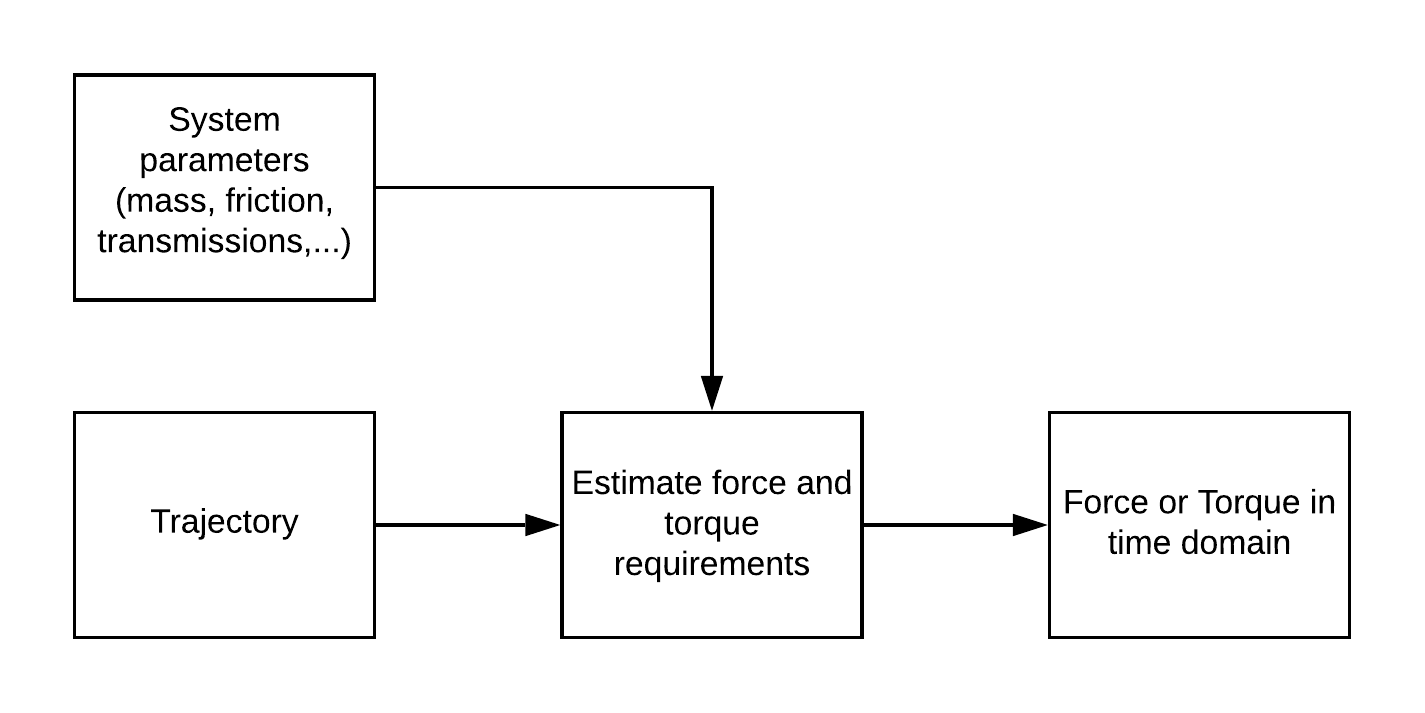
\includegraphics[width=0.5\linewidth]{./pics/forceTorque.png}
	\end{figure}

	\section{d'Alembert's principle (taking masses into account)}
	\[F=ma\]
	\[M=J \alpha \]

	\section{Static and viscous friction}
		Friction source can be focussed onto the linear guidance. Friction resulting from rotational bearing can be neglected due to very low impact of rough estimation calculation. Thus, only friction of linear guidance with ball guiding is considered and estimated. The amount of static friction is proportinal to the size and number of guide carriages. A distinction into two different sizes of guide carriages is made.
		\begin{figure}[h!]
			\centering
			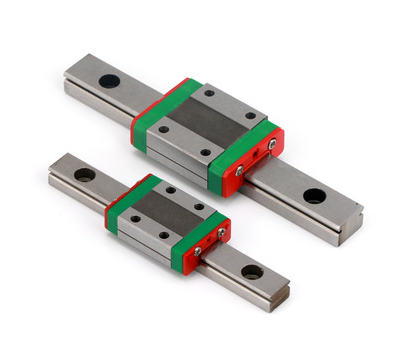
\includegraphics[width=0.3\linewidth]{./pics/linearguide.png}
			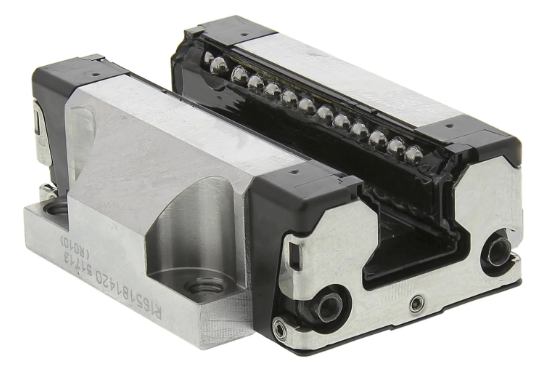
\includegraphics[width=0.25\linewidth]{./pics/ballguid.png}
			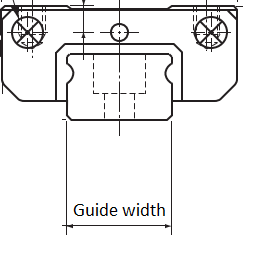
\includegraphics[width=0.2\linewidth]{./pics/guidewidth.png}
			\caption{Linear guidance with ball guiding}
		\end{figure}
		\begin{tcolorbox}[title=Friction estimation values]
			\centering
			{\def\arraystretch{2}\tabcolsep=10pt
			\begin{tabular}{c|p{3.5cm}|p{3.7cm}}
				\textbf{Guidance width} & \textbf{Static friction estimation per guide carriage} & \textbf{Viscous friction estimation per guide carriage} \\
				\hline
				$ < $ 12mm & 5 N & 15 $ \frac{N}{m/s} $\\
				$ > $ 12mm & 10 N & 30 $ \frac{N}{m/s} $\\
			\end{tabular}
			\leavevmode\\
			\begin{flushleft}
				Important: This estimated friction force is only for ONE guide carriage. Multiply it with the number of carriages you have on your axis.
			\end{flushleft}
			}
		\end{tcolorbox}
	
%			\begin{figure}[h!]
%				\centering
%				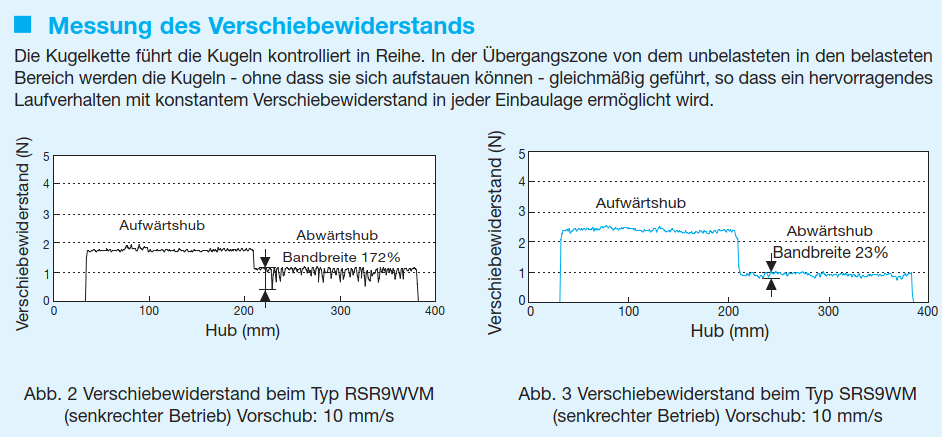
\includegraphics[width=0.8\linewidth]{./pics/thk.png}
%				\caption{Example from THK. Linear Friction of a linear guidance with guide-width of 9mm}
%			\end{figure}
		
		\subsection{Examples and measurments of designed axis}
			\subsubsection{Overview}
				\begin{table}[h!]\centering
					{\def\arraystretch{2}\tabcolsep=10pt
						\begin{tabular}{|p{2cm}|p{2.5cm}|p{2.2cm}|p{1.4cm}|p{2.3cm}|p{2.3cm}|}
							\hline
							\textbf{Axis name} & \textbf{drive typ}e & \textbf{Number and width of linear guides} & \textbf{Number of guide carriages} & \textbf{Static linear friction in N} & \textbf{Viscous linear friction in N}\\
							\hline
							Tape Feeder Camera X & indirect spindle and belt axis & 2x12mm & 4 & 35 & 120\\
							Component Shuttle X & ironless linear motor & 1x15mm & 2 & 7.5 & 15.8\\
							\hline
						\end{tabular}
				}\end{table}
			
			\paragraph{Tape Feeder Camera X (TC-Next)}\leavevmode\\
				The spindle efficiency is 99\% and can therefore be neglected for this ball screw (lead angle is $ 24.3^{\circ} $). Otherwise the measured force would not all be caused by friction of the linear guides but also from the spindle efficiency itself.
				\begin{figure}[h!]
					\centering
					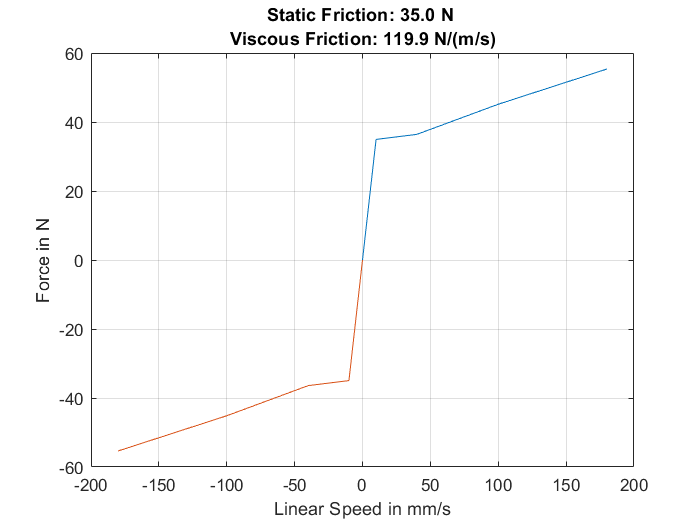
\includegraphics[width=0.49\linewidth]{./pics/firction_tapefeederX.png}
					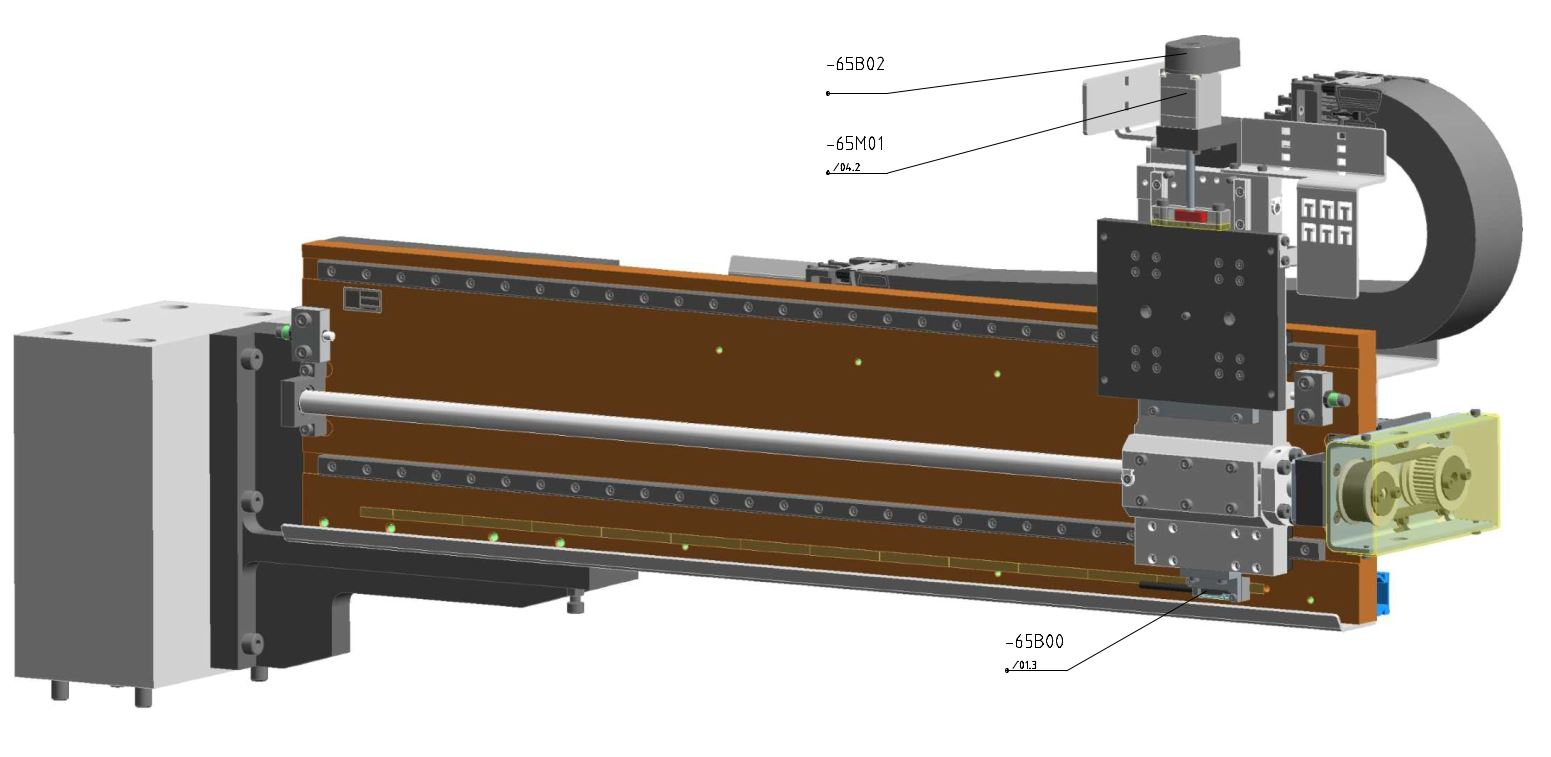
\includegraphics[width=0.45\linewidth]{./pics/tapefeederX.jpg}
					\caption{Friction plot and image of tape feeder camera axis X}
				\end{figure}
			\paragraph{Component Shuttle X (TC-Next)}\leavevmode\\
				\begin{figure}[h!]
					\centering
					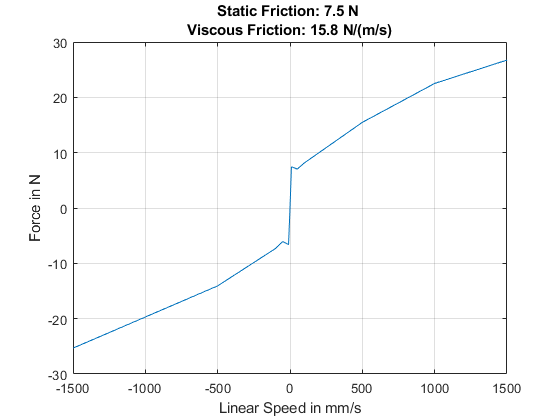
\includegraphics[width=0.49\linewidth]{./pics/friction_componentShuttleX.png}
					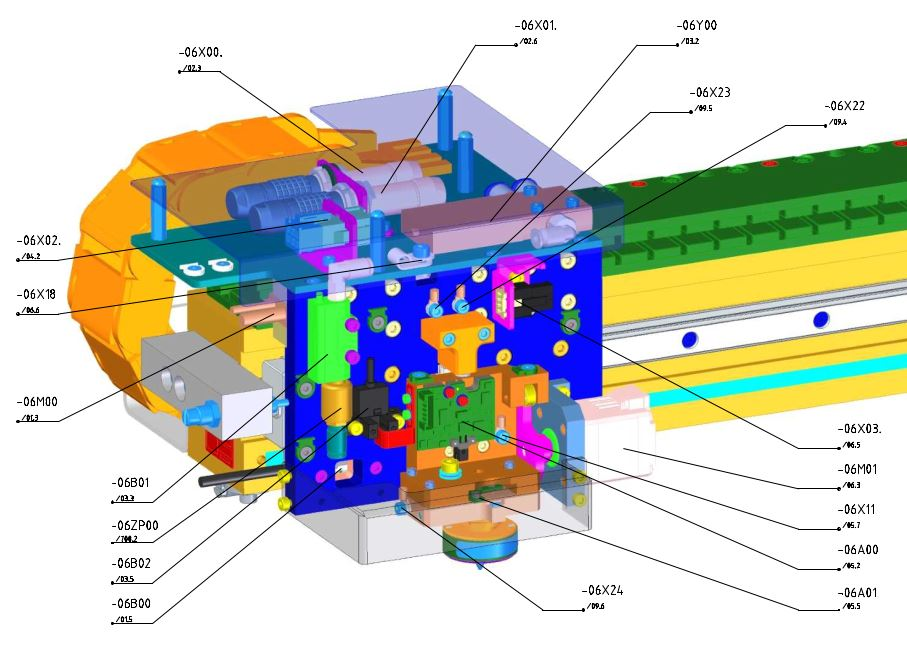
\includegraphics[width=0.45\linewidth]{./pics/componentshuttleX.jpg}
					\caption{Friction plot and image of tape component shuttle axis X}
				\end{figure}
				\clearpage
		
	\section{Spindle}
		\subsection{Efficiency}
			Basically we differentiate between Ball Screw (ger.: Kugelumlaufspindel) and Sliding-screw (ger.: Gleitspindel). The efficiency is determinded by the lead angle of the spindle.
			\begin{figure}[h!]
				\centering
				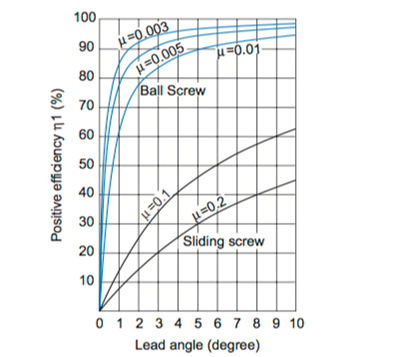
\includegraphics[width=0.5\linewidth]{./pics/spindle_efficiency.png}
				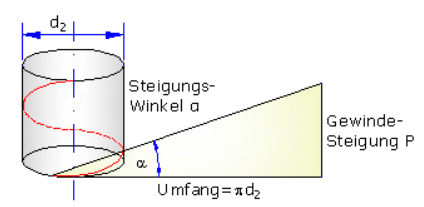
\includegraphics[width=0.49\linewidth]{./pics/leadanglecalc.png}
			\end{figure}
		
			\begin{tcolorbox}[title=Calculation of spindle lead angle]
				Lead angle is calculate by the spindle pitch and the circumference
				\[\beta=\arctan\bigg(\frac{S}{D\pi}\bigg) \]
				\tcblower
				$ \beta $ ... Lead Angle
				
				$ S $ ... Spindle pitch 
				
				$ D $ ... Spindle diameter
			\end{tcolorbox}	
		
		\subsection{Pitch accuracy}
			Basically grinded (ger.: geschliffene) spindles are more accuarte than rolled spindles. 
			\begin{table}[h!]\centering
				{\def\arraystretch{2}\tabcolsep=10pt
					\begin{tabular}{l|l}
						\textbf{Spindle type} & \textbf{Rough pitch error}\\
						\hline
						Grinded screw (ger.:Geschliffene Spindel) & $ \pm 60 \dfrac{\mu m}{m}$\\
						Rolled screw (ger.:Gerollte Spindel) & $ \pm 167 \dfrac{\mu m}{m}$\\ 
					\end{tabular}
			}\end{table}
			\begin{figure}[h!]
				\centering
				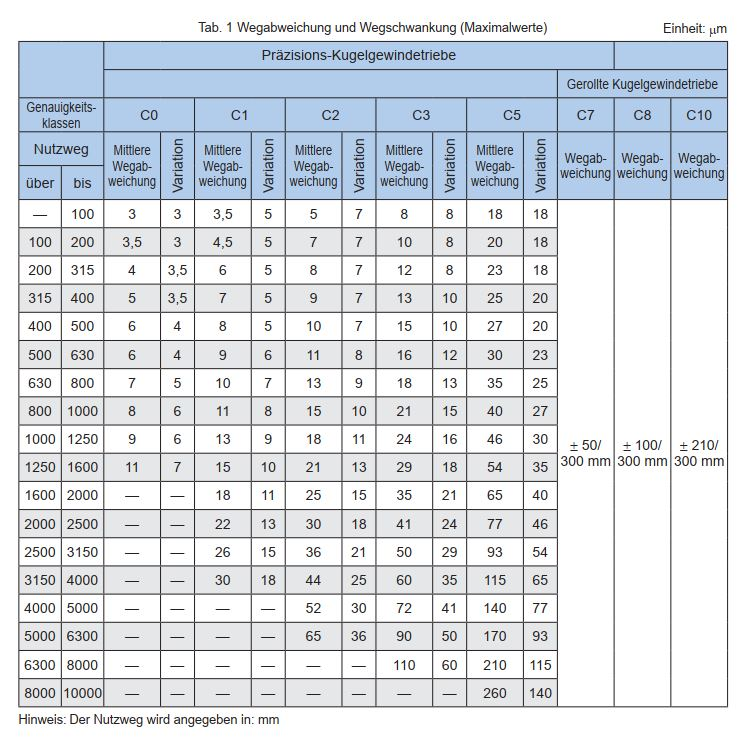
\includegraphics[width=1.0\linewidth]{./pics/spindle_accuracy.jpg}
				\caption{HIWIN accuary classes for grinded and rolled spindles}
			\end{figure}
		
\section{Summary}

	\begin{minipage}[t]{0.499\textwidth}
		\begin{tcolorbox}[title=Force/Torque]
			\textbf{Linear force:}
			\[F_{lin}=m_{lin}\cdot a + F_{r} + b_{v}\cdot v \]
			
			$ b_{v} $ ... viscous friction coefficient in $ \frac{N}{m/s} $\\
			$ F_{r} $ ... static friction force\\
			$ m_{lin} $ ... linear mass to be moved\\
			
			\textbf{Torque:}
			\[M_{rot} = M_{r} + J\cdot \alpha \]
			
			$ M_{r} $ ... friction torque in $ N $\\
			$ J $ ... moment of inertia in $ kg\cdot m^{2} $\\
			$ \alpha $ ... angular acceleration in $ \frac{rad}{s^{2}} $\\
		\end{tcolorbox}
	\end{minipage}
	\begin{minipage}[t]{0.499\textwidth}
		\begin{tcolorbox}[title=Force/Torque Transmissions]
			\textbf{Linear Force to Torque:}
			\[M_{rot} = \frac{F_{lin}\cdot S}{2\pi\cdot \eta} \]
			
			$ S $ ... spindle pitch in $ \frac{m}{turn} $\\
			$ \eta $ ... spindle efficiency\\ 
			
			\textbf{Torque to linear force:}
			\[F_{lin} = \frac{2\pi \cdot M_{rot}\cdot \eta}{S} \]
			\vspace{0.75cm}
		\end{tcolorbox}
	\end{minipage}
	
	
	\begin{tcolorbox}[title=Position/Speed/Acceleration]
		\begin{minipage}[t]{0.499\textwidth}
			\textbf{Transmission Linear to rotational}
			\[\phi=2\pi \cdot\frac{s}{S} \]
			\[\omega=2\pi \cdot\frac{v}{S} \]
			\[\alpha=2\pi \cdot\frac{a}{S} \]
			$ \phi $ ... Rotional position in $ rad $\\
			$ \omega $ ... Rotational speed in $ \frac{rad}{s} $\\
			$ \alpha $ ... Rotational acceleration in $ \frac{rad}{s^{2}} $\\
			$ S $ ... spindle pitch in $ \frac{m}{turn} $\\
		\end{minipage}
		\begin{minipage}[t]{0.499\textwidth}
			\textbf{Transmission Rotational to linear}
			\[s=\frac{\phi\cdot S}{2\pi} \]
			\[v=\frac{\omega\cdot S}{2\pi} \]
			\[a=\frac{\alpha\cdot S}{2\pi} \]
			
			$ s $ ... Linear position in $ m $\\
			$ v $ ... Linear speed in $ \frac{m}{s} $\\
			$ a $ ... Linear acceleration in $ \frac{m}{s^{2}} $\\
		\end{minipage}

		\textbf{Number of revolutions}
		\[n = \frac{\omega \cdot 60}{2 \cdot \pi} \]
		$ n $ ... number of revolutions in $ rpm $
	\end{tcolorbox}

	\begin{tcolorbox}[title=Motor related]
		\textbf{Force constant}
		\[k_{t}= \frac{M_{stall}}{I_{max}} \]
		$ k_{t} $ ... force constant in $ \frac{Nm}{Arms} $\\
		$ I_{max} $ ... maximum current in $ Arms $\\
		
		\textbf{Continuous current}
		\[I_{cont} = \frac{M_{mean}}{k_{t}}\]
		$ I_{cont} $ ... contiuous current in $ Arms $\\
		$ M_{mean} $ ... mean torque of trajectory in $ Nm $\\
		

	\end{tcolorbox}


	\part{Stepper-Motor-Design}
	
	\part{Linear-Motor-Design}
\end{document}